\chapter{Photons and the Future of Physics}
\setcounter{section}{7}
\setcounter{subsection}{0}
\setcounter{subsubsection}{1}
\setcounter{secnumdepth}{3}
% Box styles
\tcbset{physikbox/.style={colback=blue!5!white, colframe=blue!75!black, fonttitle=\bfseries}}
\tcbset{mathebox/.style={colback=green!5!white, colframe=green!50!black, fonttitle=\bfseries}}
\tcbset{didaktikbox/.style={colback=yellow!5!white, colframe=yellow!50!black, fonttitle=\bfseries}}
\tcbset{hypobox/.style={colback=orange!5!white, colframe=orange!75!black, fonttitle=\bfseries}}
\tcbset{hinweisbox/.style={colback=gray!10!white, colframe=black!40!black, fonttitle=\bfseries}}

\subsection{Introduction}
\index{Photon}
\index{Photonics}
\index{Communication}
\index{Metrology}
\index{Data processing}
\index{Photonic computer}
\index{Quantum communication network}
\index{Graviton}
\index{Dark energy}
\index{Standard Model}

Photons not only shape today’s technology but also open doors to entirely new areas of research.  
While they are already indispensable in communication, metrology, and data processing, we are also at the beginning of an era in which photons take on central roles in photonic computers, quantum communication networks, and the most precise experiments in fundamental physics.  
This chapter spans the arc from current developments in photonics to forward-looking applications and the great open questions of physics — from the search for the hypothetical graviton, to the puzzle of dark energy, to possible extensions of the Standard Model.  
The topics presented show how the smallest quantum of light could become the key to the technologies and discoveries of tomorrow.
\newpage
\noindent
\begin{figure}[H]
	\centering
	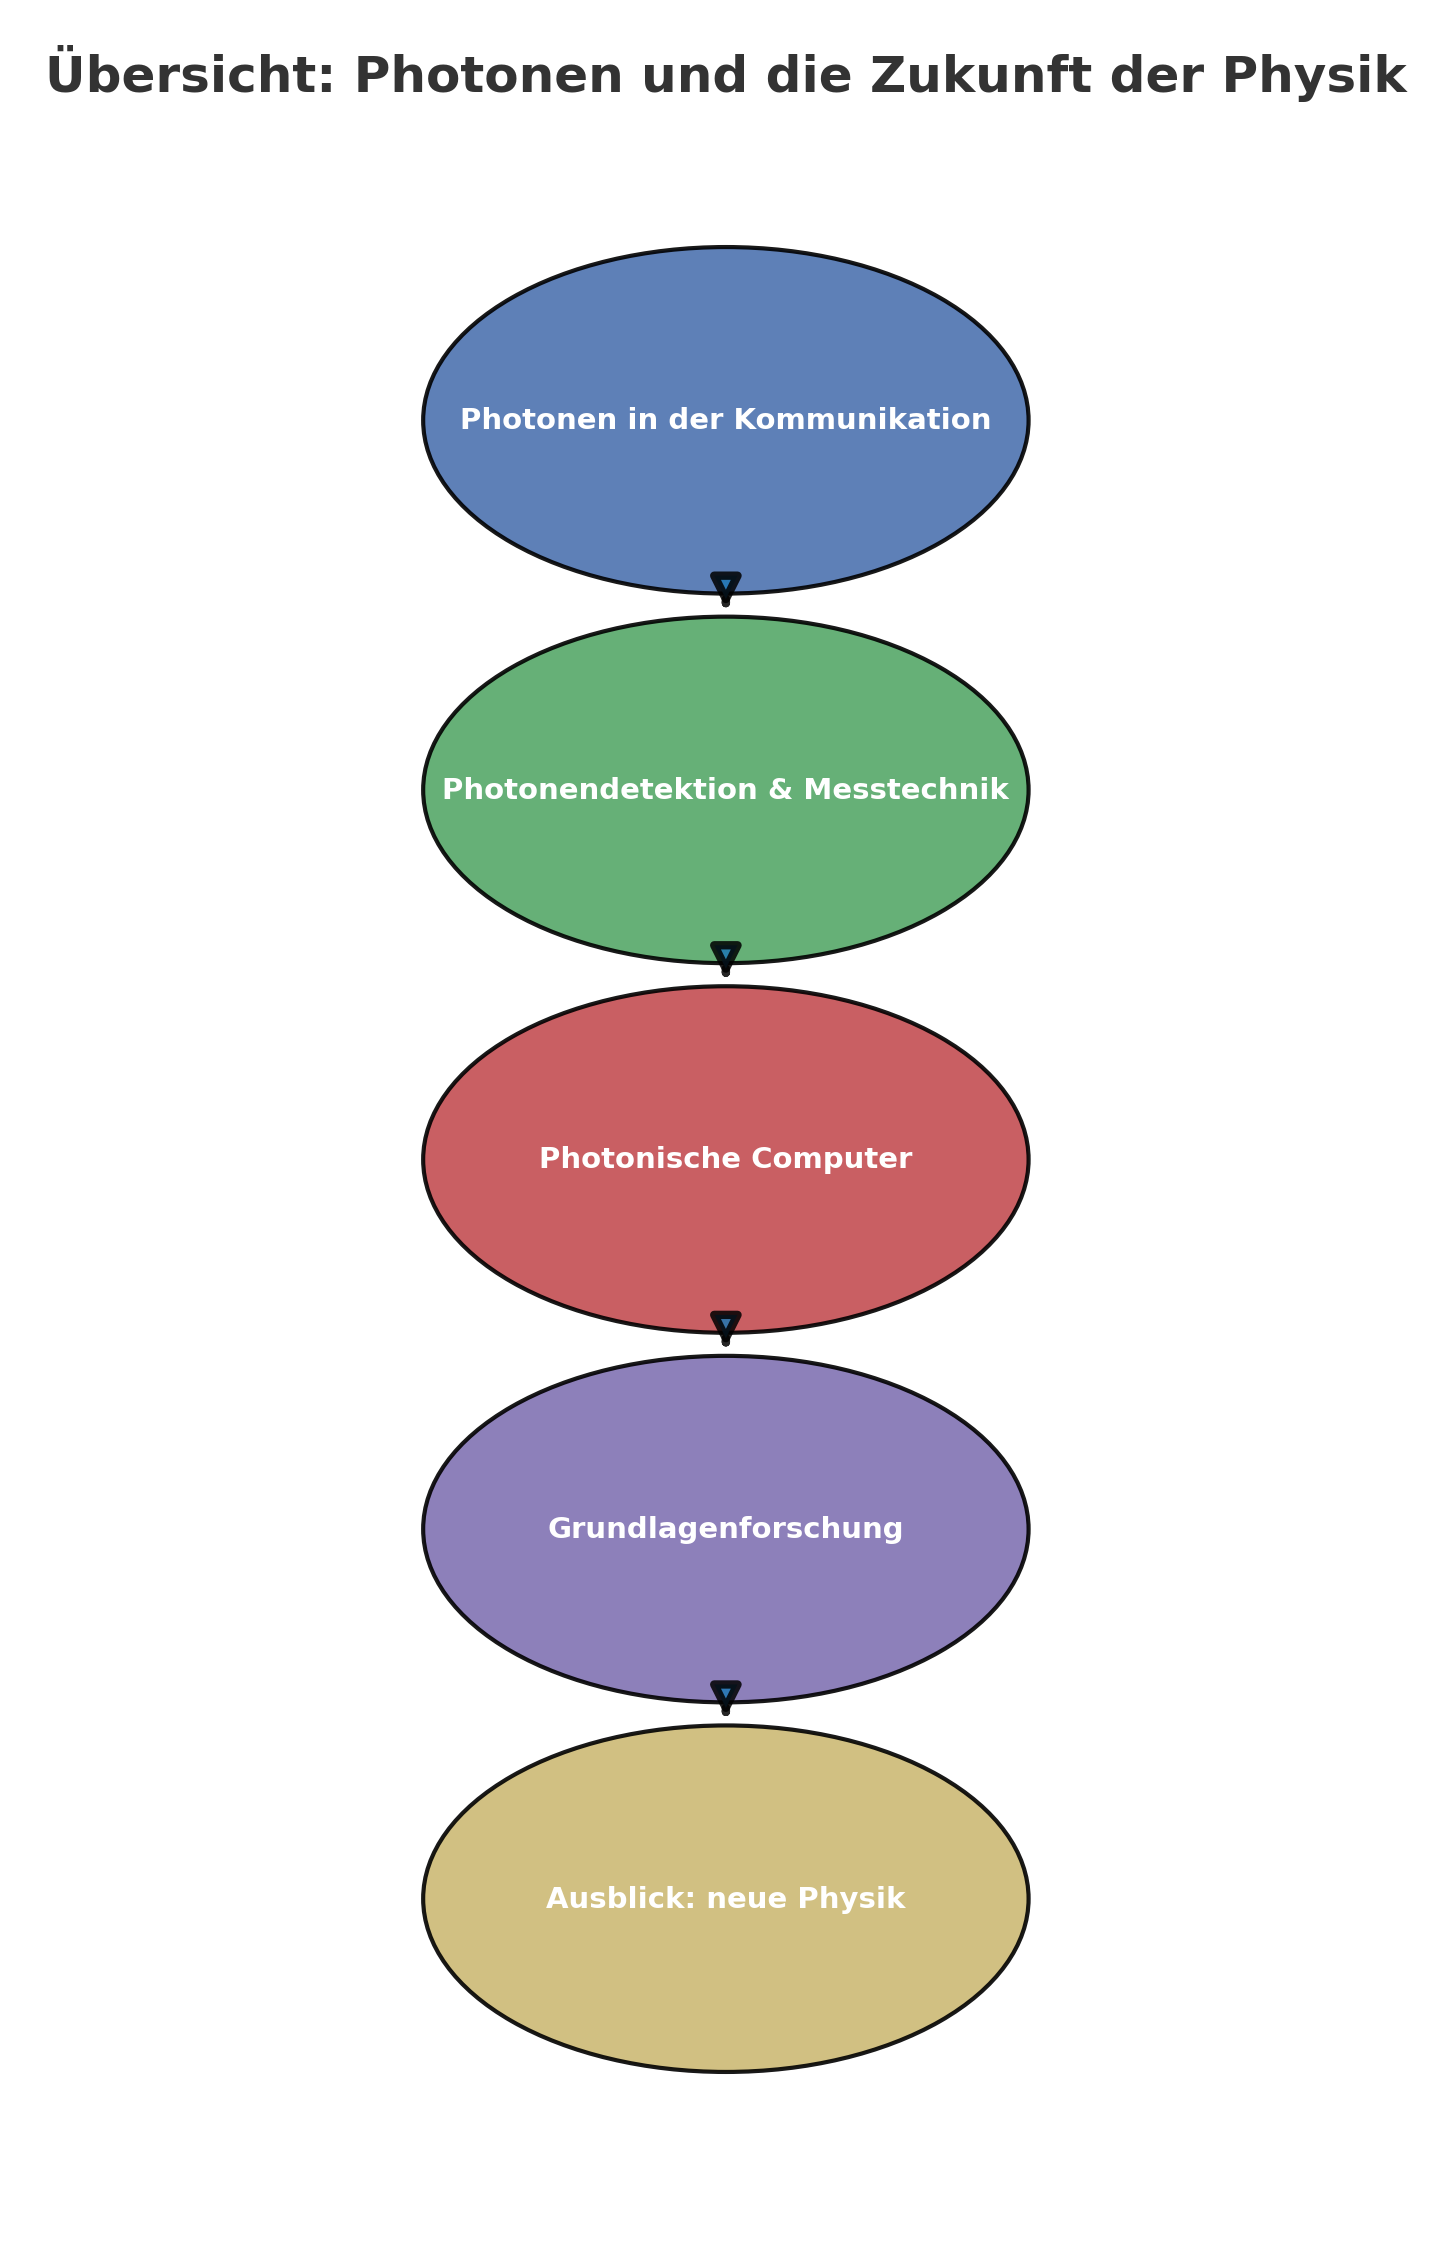
\includegraphics[width=0.75\textwidth]{bilder/kapitel_VII_uebersicht.png}
	\caption[Overview Chapter~VII]{Overview: Photons and the Future of Physics. 
		The graphic shows the main themes of this chapter in a vertical arrangement, 
		from photonic logic to open questions of new physics.}
	\label{fig:kapitel_VII_uebersicht}
\end{figure}

\subsection{Single Photons and Quantum Information}
\index{Single photon}
\index{Quantum information}
\index{Qubit}
\index{Superposition}
\index{Polarization}
\index{Time-bin}
\index{Frequency encoding}

The ability to generate, control, and detect individual photons has taken on a key role in quantum information technology in recent years. Single photons serve as ideal carriers of quantum information: they are robust against disturbances, travel at the speed of light\index{Speed of light}, and can be prepared in well-defined quantum states\index{Quantum state}.

In classical information technology, bits are stored and processed in the form of electrical voltages or magnetic states. In quantum information, by contrast, the smallest unit — the \emph{qubit} — is based on the coherent superposition\index{Superposition} of states. For photons, these states are often realized through polarization directions, time bins, or path information.
\vspace{1em}
\begin{tcolorbox}[physikbox, title=What Makes a Photon an Information Carrier? \label{box:photon_information}]
	\small
	Photons can carry different physical degrees of freedom that are usable as qubits:
	\begin{itemize}
		\item \textbf{Polarization:} Horizontal ($\ket{H}$) and vertical ($\ket{V}$) as basis states.
		\item \textbf{Time bins:} Early and late arrival times as logical states.
		\item \textbf{Path:} Two different optical paths in an interferometer\index{Interferometer}.
		\item \textbf{Frequency:} Different spectral modes for encoded information.
	\end{itemize}
	These degrees of freedom can be precisely controlled and transmitted over long distances without destroying the quantum information.
\end{tcolorbox}

\subsubsection{Generation of Single Photons}
\index{Single-photon source}
\index{Spontaneous parametric down-conversion}
\index{Single atom}
\index{Ion}
\index{Quantum dot}
\index{Nonlinear crystal}
\index{Semiconductor material}

Single-photon sources are central building blocks of quantum optics\index{Quantum optics}. Common methods include:
\begin{itemize}
	\item \emph{Spontaneous parametric down-conversion} (SPDC) in nonlinear crystals.
	\item \emph{Single atoms} or ions in optical traps\index{Optical trap}.
	\item \emph{Quantum dots} in semiconductors.
\end{itemize}
The goal is to generate photons with high purity (low multi-photon probability) and high indistinguishability.
\newpage
\noindent
\vspace{1em}
\begin{tcolorbox}[hinweisbox, title=What Does “Indistinguishability” Mean? \label{box:indistinguishability}]
	\small
	In quantum optics, \emph{indistinguishability} means that two photons are identical in all physical properties:
	\begin{itemize}
		\item same frequency (energy)
		\item same polarization
		\item identical spatial mode (same optical path)
		\item identical arrival time within the coherence time
	\end{itemize}
	Only if photons are perfectly indistinguishable can they exhibit quantum interference effects such as the \emph{Hong–Ou–Mandel dip}.
\end{tcolorbox}
\vspace{1em}
\begin{tcolorbox}[physikbox, title=The Hong–Ou–Mandel Dip Phenomenon \label{box:hong_ou_mandel}]
	\small
	The \emph{Hong–Ou–Mandel dip} experiment is a central method for verifying the \emph{indistinguishability} of two photons. When two indistinguishable photons simultaneously strike a 50:50 beam splitter, they always leave it together through the same output — a purely quantum interference effect.  
	The depth of the measured “dip” in the coincidence rate is a direct measure of the indistinguishability of the photons.  
	A detailed description and figure can be found in \textbf{Chapter IV.5}.
\end{tcolorbox}

\subsubsection{Decoherence and Sources of Error}
\index{Decoherence}
\index{Quantum error correction}
\index{Quantum repeater}
\index{Fiber attenuation}
\index{Scattering}
\index{Phase noise}
\index{Vibration}

Quantum information is sensitive to disturbances. For photons, the main causes of decoherence are:
\begin{itemize}
	\item Interaction with the transmission medium (e.g., fiber attenuation, scattering).
	\item Phase noise due to temperature fluctuations and vibrations.
\end{itemize}
Error correction and quantum repeaters are necessary to preserve quantum information over long distances.
\newpage
\noindent
\subsubsection{Applications}
\index{Quantum cryptography}
\index{Satellite communication}
\index{Hybrid quantum system}

Single photons form the basis for:
\begin{itemize}
	\item Quantum cryptography.
	\item Quantum communication via satellites.
	\item Hybrid systems in which photons serve as interfaces between matter qubits.
\end{itemize}
These applications mark the beginning of a new era of information processing, in which photons are not only carriers but also mediators between different quantum systems.

\subsection{Quantum Cryptography and  Quantum\newline Communication} \label{sec:quantum_crypto}
\index{RSA}
\index{Quantum computer}
\index{Quantum cryptography}
\index{Quantum communication}
\index{Heisenberg uncertainty principle}
\index{No-cloning theorem}
\index{BB84 protocol}
\index{Bennett, Charles}
\index{Brassard, Gilles}
\index{Quantum key distribution}
\index{Satellite-based quantum communication}
\index{Micius}

The security of classical communication systems is based on mathematical methods whose safety relies on the practical impossibility of certain computations — such as factoring large numbers in RSA. This security may be threatened by future quantum computers.  
Quantum cryptography, on the other hand, uses fundamental physical laws to ensure security — independent of an attacker’s computational power.
\vspace{1em}
\begin{tcolorbox}[physikbox, title=Core Principle of Quantum Cryptography \label{box:qcrypto_prinzip}]
	\small
	Quantum cryptography rests on two central features of quantum mechanics:
	\begin{enumerate}
		\item \textbf{Measurement disturbance:} Any attempt to measure a quantum state changes it (Heisenberg uncertainty principle).
		\item \textbf{No cloning:} Unknown quantum states cannot be copied without error (no-cloning theorem).
	\end{enumerate}
	Thus: eavesdropping inevitably leaves traces that can be detected by the legitimate communication partners.
\end{tcolorbox}
\newpage
\noindent
\subsubsection{Quantum Key Distribution (QKD)}

The best-known protocol is \textbf{BB84} (Bennett \& Brassard, 1984). Here, single photons are transmitted in random polarization states.  
The process in short:
\begin{itemize}
	\item Sender (\emph{Alice}) randomly chooses one of two possible bases (e.g., horizontal/vertical or diagonal).
	\item Receiver (\emph{Bob}) measures in randomly chosen bases.
	\item After the transmission, both compare their basis choices publicly and discard measurements where the bases don’t match.
	\item From the remaining data, a shared key is extracted.
\end{itemize}
An eavesdropper (\emph{Eve}) introduces extra errors that can be detected statistically.

\subsubsection{Quantum Communication over Large Distances}

The range of direct quantum communication is limited by losses in optical fibers\index{Fiber optics} and atmospheric disturbances\index{Atmosphere}. Possible solutions include:
\begin{itemize}
	\item \textbf{Quantum repeaters:} Nodes that generate entangled photon pairs\index{Entangled photons} and distribute them over large distances.
	\item \textbf{Satellite-based quantum communication:} Avoiding fiber losses by free-space transmission (e.g., the Chinese quantum communication satellite \emph{Micius}).
\end{itemize}

\subsubsection{Applications and Outlook}

Quantum cryptography is currently being tested for highly secure government and financial communications. In combination with classical networks, hybrid systems are emerging that will enable long-term secure communication even in the age of quantum computers.

Remarkably, quantum physics plays a double role here:  
On one hand, quantum computers threaten the security of today’s encryption methods through their computational power.  
On the other, the very same physics provides with quantum cryptography an entirely new approach that allows in principle eavesdrop-proof communication.  
This interplay between challenge and solution makes quantum communication one of the most exciting research fields in modern physics.

\subsection{Photonics as a Future Technology}
\index{Laser}
\index{LED}
\index{Fiber optics}
\index{Photonic chip}
\index{Photon detector}
\index{Modulator}
\index{Filter}
\index{Nonlinear crystal}

Photons are not only fundamental carriers of information in quantum physics but also the basis of numerous modern technologies.  
\emph{Photonics} encompasses all technologies based on the generation, control, and detection of light — from lasers in medicine to fiber optics in global communication networks.
\vspace{1em}
\begin{tcolorbox}[hinweisbox, title=What Does “Photonics” Mean? \label{box:photonics_definition}]
	\small
	The term \emph{photonics} describes the engineering and technological use of photons — analogous to electronics, which deals with electrons.  
	Photonics includes:
	\begin{itemize}
		\item Light sources (lasers, LEDs, quantum light sources)
		\item Light guidance (fiber optics, photonic chips)
		\item Light detection (cameras, photon detectors)
		\item Light manipulation (modulators, filters, nonlinear crystals)
	\end{itemize}
\end{tcolorbox}

\subsubsection{Photonics in Communication}
\index{Telecommunication}
\index{Photonic switch}
\index{Router}
\index{Microchip}

In telecommunications, photonics is increasingly replacing electronics to handle the growing volumes of data. Fiber networks transmit information at the speed of light with minimal energy loss.  
Photonic switches and routers on microchips promise ultra-fast signal processing directly with photons.

\subsubsection{Photonics in Medicine}
\index{Laser surgery}
\index{Optical coherence tomography}
\index{Fluorescence diagnostics}
\index{Biosensor}

Photon-based methods such as laser surgery, optical imaging (OCT), and fluorescence diagnostics have revolutionized medicine.  
Future developments include minimally invasive operations with ultrashort laser pulses and photonic biosensors for real-time diagnostics.

\subsubsection{Photonics in Sensing and Metrology}
\index{Photonic sensor}
\index{LIDAR}
\index{Gravitational-wave detector}

Photonic sensors enable high-precision measurements in industry, geoscience, and space research.  
Examples include LIDAR systems for autonomous driving and interferometric gravitational-wave detectors.
\newpage
\noindent
\vspace{1em}
\begin{tcolorbox}[physikbox, title=Photonic Circuits vs. Electronic Circuits \label{box:photon_vs_electron}]
	\small
	Photonic circuits offer several decisive advantages over electronic approaches:
	\begin{itemize}
		\item \textbf{Higher speed:} Light moves through a medium much faster than electrons through conductors.
		\item \textbf{Lower losses:} No ohmic heating from electrical resistance.
		\item \textbf{Greater bandwidth:} A photon signal can carry many wavelengths simultaneously (multiplexing).
		\item \textbf{Low crosstalk:} Hardly any electromagnetic interference between adjacent lines.
	\end{itemize}
	These features make photonic circuits a key factor for future high-speed and high-bandwidth technologies.
\end{tcolorbox}

\subsubsection{Outlook}

Photonics is considered a key technology of the 21st century. Its combination with quantum physics — in quantum communication, quantum computers, or quantum metrology — promises entirely new applications.  
The development toward integrated photonic circuits could trigger a transformation in information processing similar to that of microelectronics in the 20th century.

\subsection{Optical Logic and Photonic Computers}
\index{Optical logic}
\index{Mach--Zehnder interferometer}
\index{Microresonator}
\index{Optical modulator}

The miniaturization of electronic circuits is increasingly reaching physical limits: transistors are becoming so small that quantum and thermal effects impair their function. At the same time, the energy demand of modern data centers is rising rapidly. A promising alternative is to use photons instead of electrons for information processing.
\newpage
\noindent
\vspace{1em}
\begin{tcolorbox}[physikbox, title=Why Photons Are Attractive for Logic Circuits, label=box:optlogik_vorteile]
	\small
	\begin{itemize}
		\item \textbf{High speed:} Light moves nearly at the speed of light — optical signals can be processed extremely fast.
		\item \textbf{No ohmic losses:} Unlike electric currents, optical lines hardly heat up.
		\item \textbf{Parallel processing:} Multiple wavelengths can be used simultaneously through multiplexing.
		\item \textbf{Direct coupling to fiber communication:} No conversion between electron and photon signals needed.
	\end{itemize}
\end{tcolorbox}

\subsubsection{Basic Principle of Optical Logic Gates}
\index{Optical logic gate}
\index{Photonic crystal}

Optical logic circuits work with components that redirect, attenuate, or amplify light beams depending on input conditions. Examples include nonlinear crystals, optical modulators, or photonic crystal structures.  
Logic gates such as \textsc{AND}, \textsc{OR}, and \textsc{NOT} can be realized via interference, absorption, or polarization changes.
\vspace{1em}
\begin{tcolorbox}[didaktikbox, title=From Electronics to Photonics]
	\label{box:optlogik_didaktik}
	\small
	In electronics, logic gates are based on transistors that block or allow current flow. In photonics, components such as Mach–Zehnder interferometers or microresonators take on this role — but for light.
\end{tcolorbox}

\subsubsection{Photonic Computers}
\index{Photonic computer}
\index{Artificial intelligence}
\index{Signal processing}
\index{Quantum information processing}

A photonic computer uses optical circuits for central computational operations. This technology is particularly suitable for:
\begin{itemize}
	\item \textbf{Artificial intelligence:} Matrix multiplications can be carried out extremely fast and energy-efficiently in optical networks.
	\item \textbf{Signal processing:} Broadband processing without electrical bottlenecks.
	\item \textbf{Quantum information processing:} Combination of photonic logic and quantum bits (qubits).
\end{itemize}
\vspace{1em}
\begin{tcolorbox}[hypobox, title={What If Optical Computers Replaced Electronics?}]
	\label{box:optlogik_zukunft}
	\small
	If photonic computers could fully replace electronics, the energy consumption of large data centers could be drastically reduced. At the same time, clock rates in the terahertz range might be achieved — far beyond today’s processors.
\end{tcolorbox}

Optical logic gates can also be realized with a Mach–Zehnder interferometer (MZI). 
A beam splitter divides the laser beam into two paths, each containing a phase modulator. 
Only if both modulators apply a certain phase shift do the beams interfere at the second beam splitter in such a way that light appears at the desired output. 
Choosing the phases so that this happens only when both inputs are active makes the MZI work like a classical \textsc{AND} gate — but in a purely optical way. 
\vspace{1em}
\begin{tcolorbox}[didaktikbox, title=Photonic AND Gate in a Mach--Zehnder Interferometer, label={box:mzi_and}]
	\small
	A Mach--Zehnder interferometer can be configured to work as an \textsc{AND} gate. 
	The inputs \(A\) and \(B\) control phase modulators in the two arms of the interferometer. 
	Only if both apply a phase shift of \(\pi\), the phases add up to \(2\pi\), resulting in constructive interference at the “1” output.
	
\begin{center}
	\begin{tabular}{c c c c c c}
		\hline
		\(A\) & \(B\) & Phase A & Phase B & Output “1” & Output “0” \\
		\hline
		0 & 0 & \(0\) & \(0\) & 1 & 0 \\
		0 & 1 & \(0\) & \(\pi\) & 0 & 1 \\
		1 & 0 & \(\pi\) & \(0\) & 0 & 1 \\
		1 & 1 & \(\pi\) & \(\pi\) & 1 & 0 \\
		\hline
	\end{tabular}
\end{center}

	Only for \(A=1\) and \(B=1\) is the total phase \(2\pi\), so the upper output becomes bright. 
	In all other cases, the light is directed into the “0” output.
\end{tcolorbox}
\newpage
\noindent
\begin{figure}[H]
	\centering
	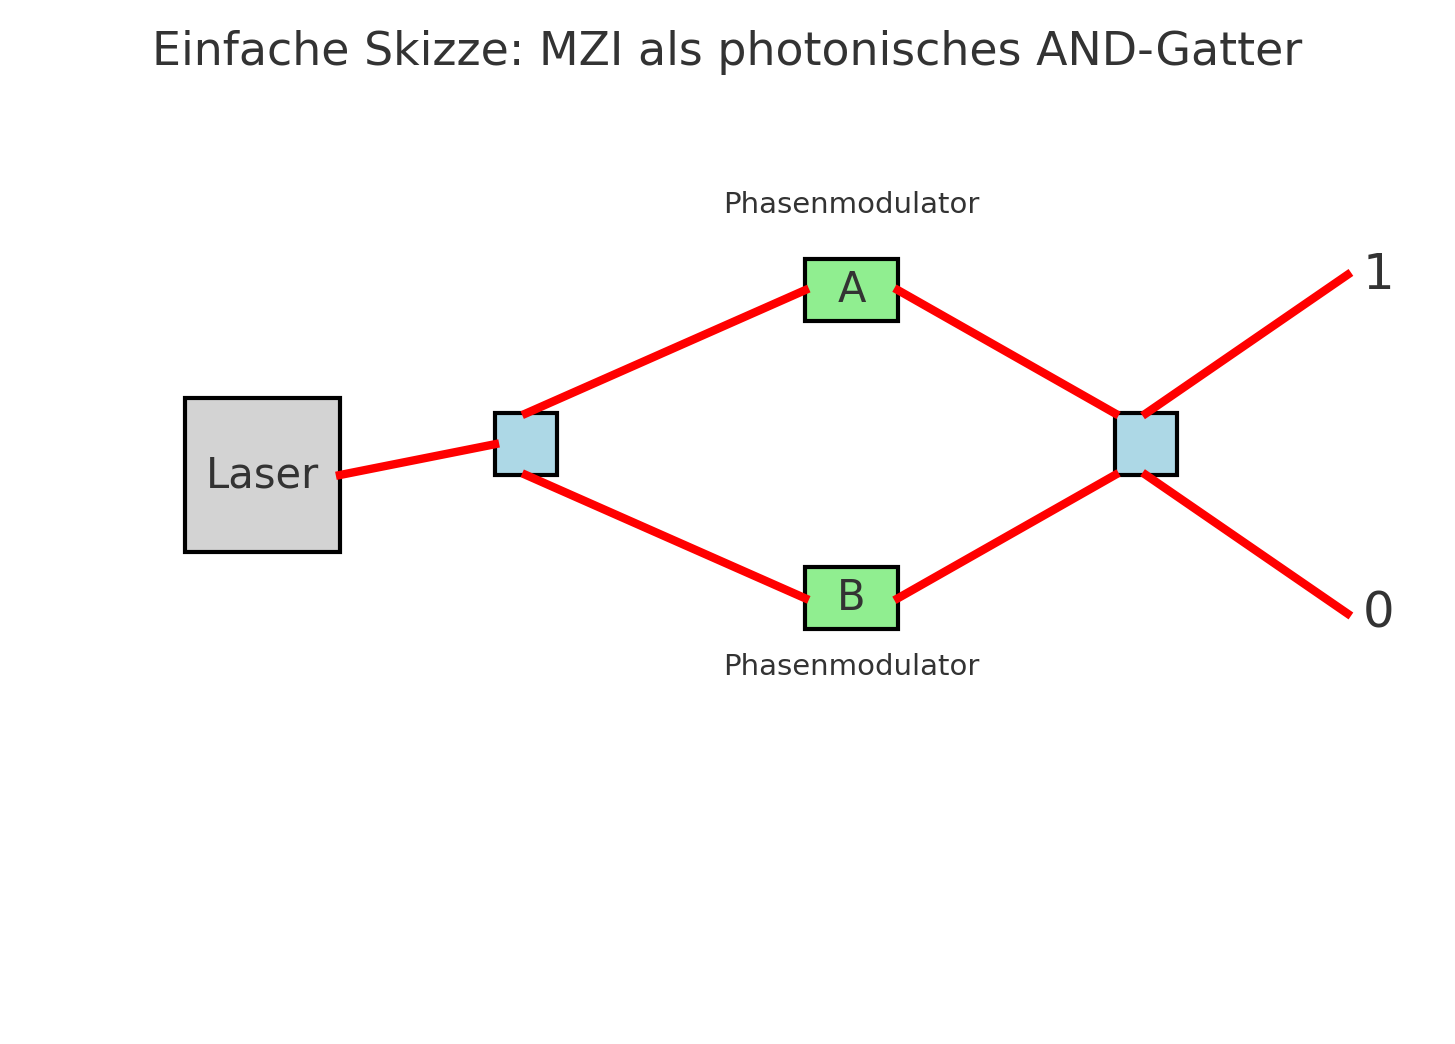
\includegraphics[width=0.75\textwidth]{bilder/mzi_and_simple.png}
	\caption{Simple schematic of a Mach--Zehnder interferometer with two phase modulators (\(A\) and \(B\)) acting as a photonic \textsc{AND} gate. Only if both modulators apply a phase shift of \(\pi\), the phases add to \(2\pi\) and light appears at the “1” output.}
	\label{fig:mzi_and_simple}
\end{figure}

\subsubsection{Challenges}
\index{Chip integration}
\index{Miniaturization}
\index{Electronics integration}

Despite the advantages, several open problems remain:
\begin{itemize}
	\item Efficient generation and control of single photons on a chip.
	\item Miniaturization of optical components to the nanometer scale.
	\item Integration with existing electronics.
\end{itemize}

\subsubsection{Summary}

Optical logic and photonic computers offer a fascinating possibility to increase computing power and reduce energy demand. Whether they will completely replace classical electronics or dominate only in special applications depends on solving the technical challenges.

\newpage
\noindent
\subsection{Photons in Fundamental Research}
\index{Boson}
\index{Cosmology}
\index{Cosmic microwave background}
\index{Bell test}
\index{Quantum tomography}
\index{Gravitational lens}
\index{Lorentz invariance}
\index{CPT symmetry}

Photons play a central role not only in technology but also in modern fundamental research. 
Their properties as massless, bosonic quantum objects make them ideal tools for studying fundamental questions of physics — from the smallest scales of quantum mechanics to cosmological distances.

\begin{itemize}
	\item \textbf{Testing quantum mechanics:} Experiments with single photons — such as double-slit experiments, Bell tests, or quantum tomography — test the limits and predictions of quantum mechanics with the highest precision.
	\item \textbf{Astrophysics and cosmology:} Photons from distant galaxies and the cosmic microwave background provide information on the origin and evolution of the universe.
	\item \textbf{Precision measurements:} Laser interferometers such as LIGO or Virgo detect tiny changes in length caused by gravitational waves — based on coherent photon beams.
	\item \textbf{Tests of fundamental symmetries:} Polarization, frequency, and flight time of photons are used to probe Lorentz invariance, CPT symmetry, and other fundamental principles.
\end{itemize}
\vspace{1em}
\begin{tcolorbox}[physikbox, title={Photons as Messengers of Natural Laws}, label={box:photonen_grundlagen}]
	\small
	Photons interact only weakly with their environment, move at the speed of light, and carry information about their source across billions of years and light-years.  
	This makes them unique messengers that provide insights into processes neither directly accessible nor reproducible — from the first moments after the Big Bang to the subtlest effects in quantum field theory.
\end{tcolorbox}
\newpage
\noindent
\begin{figure}[H]
	\centering
	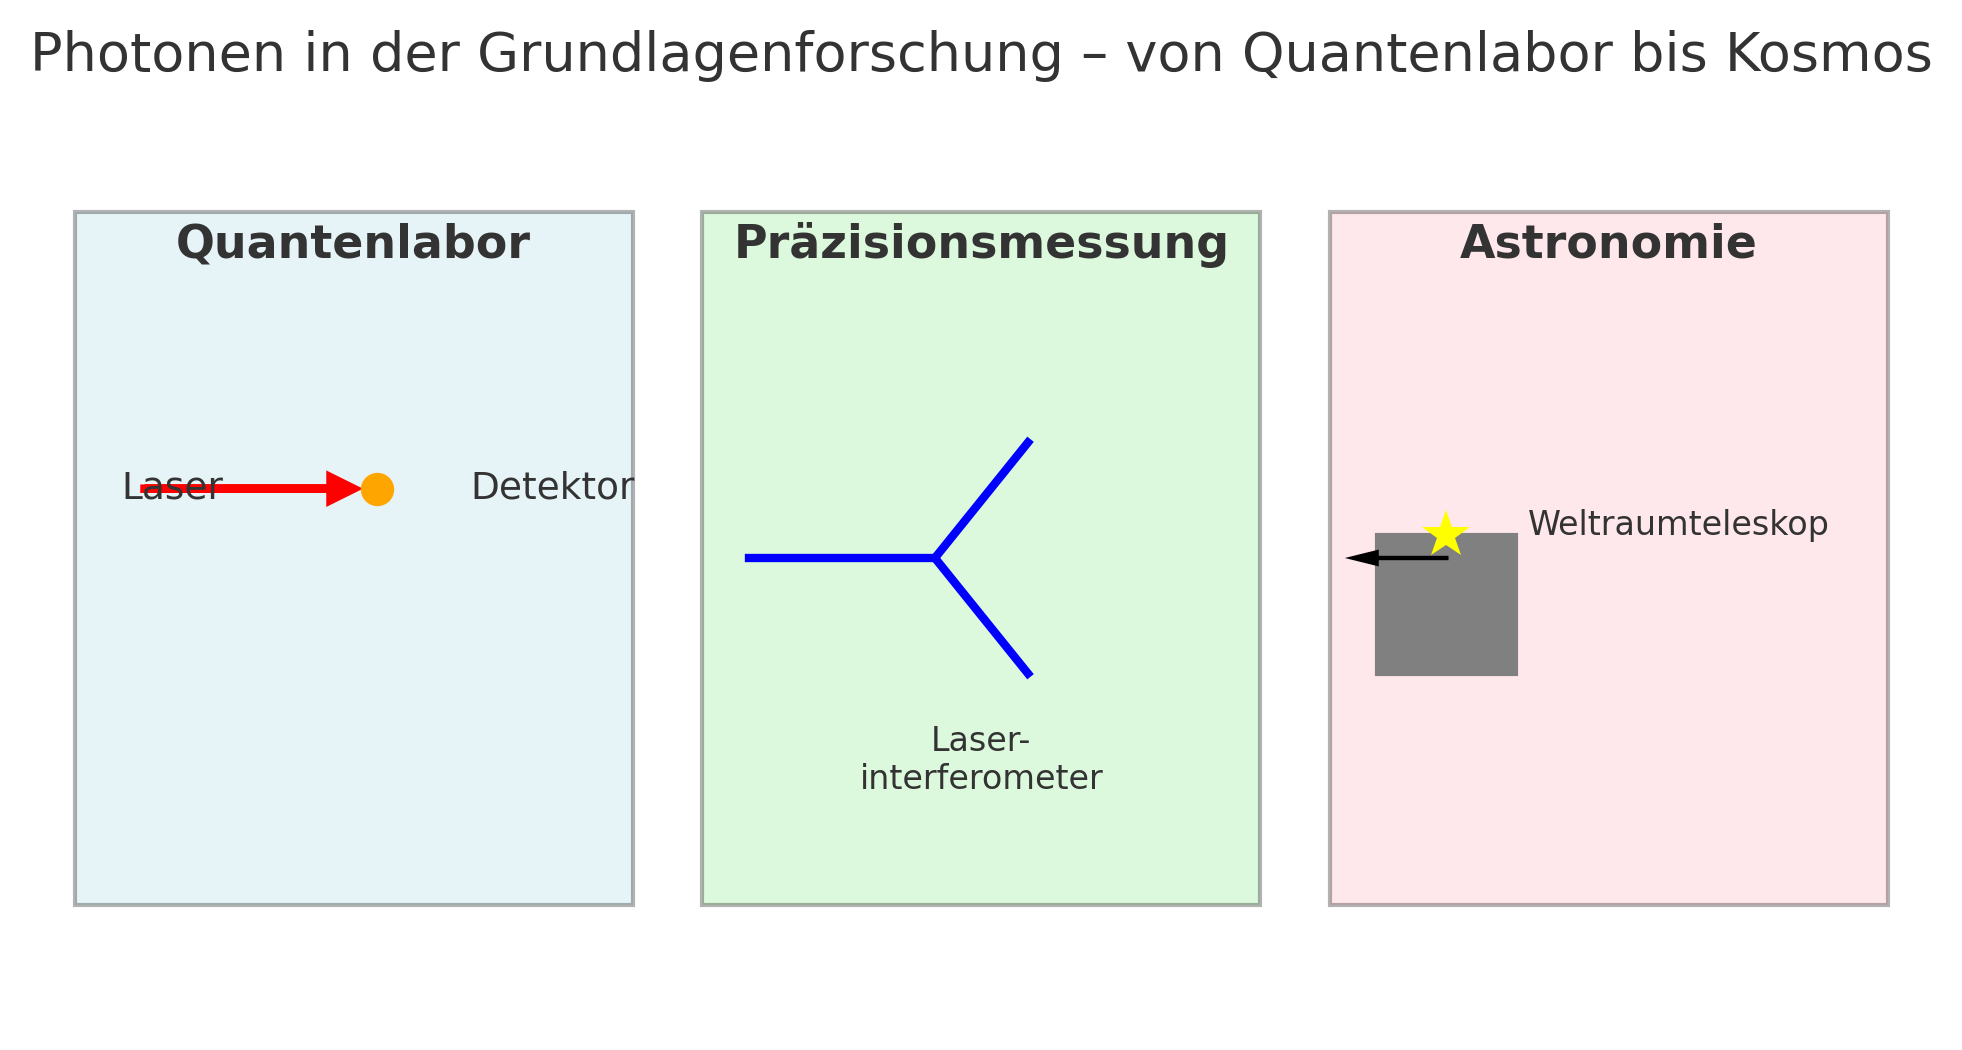
\includegraphics[width=0.9\textwidth]{bilder/photonen_grundlagenforschung.png}
	\caption{Photons in fundamental research: 
		from quantum labs and precision measurements to astronomy. 
		The illustration shows central fields of application: 
		experiments with single photons in the lab, laser interferometry for gravitational-wave detection, and space-based observations of stars and galaxies.}
	\label{fig:photonen_grundlagen}
\end{figure}

\subsubsection{Outlook}

Fundamental research with photons is far from complete. 
New detection methods, improved sources for single and entangled photons, and space-based experiments promise even deeper insights into the structure of natural laws.


\subsection{Outlook: Graviton, Dark Energy,\newline New Physics?}
\index{New physics}

Even though the photon as the quantum of light is well understood in modern physics, many fundamental questions remain — and photons often play a key role in answering them.

\begin{itemize}
	\item \textbf{The graviton:} The hypothetical exchange particle of gravitation has not yet been observed. Precise measurements with photons — via gravitational lenses or interferometry — could provide indirect evidence.
	\item \textbf{Dark energy:} The accelerated expansion of the universe points to an as-yet unknown form of energy. Photometry and spectroscopy of distant supernovae and galaxies use photons as the only information source to study this mysterious component.
	\item \textbf{New physics beyond the Standard Model:} High-precision experiments with photons could reveal deviations from established theories, such as tiny violations of Lorentz invariance or hints of additional spatial dimensions.
\end{itemize}

\begin{tcolorbox}[hypobox, title={What If the Photon Were Not the Only Massless Boson?}, label={box:photon_neue_physik}]
	\small
	The existence of additional massless exchange particles — such as the graviton — would fundamentally change our understanding of the fundamental forces.  
	Photon experiments could, through subtle effects such as deviations in light propagation or polarization patterns, provide the first hints of such new physics.
\end{tcolorbox}
\begin{figure}[H]
	\centering
	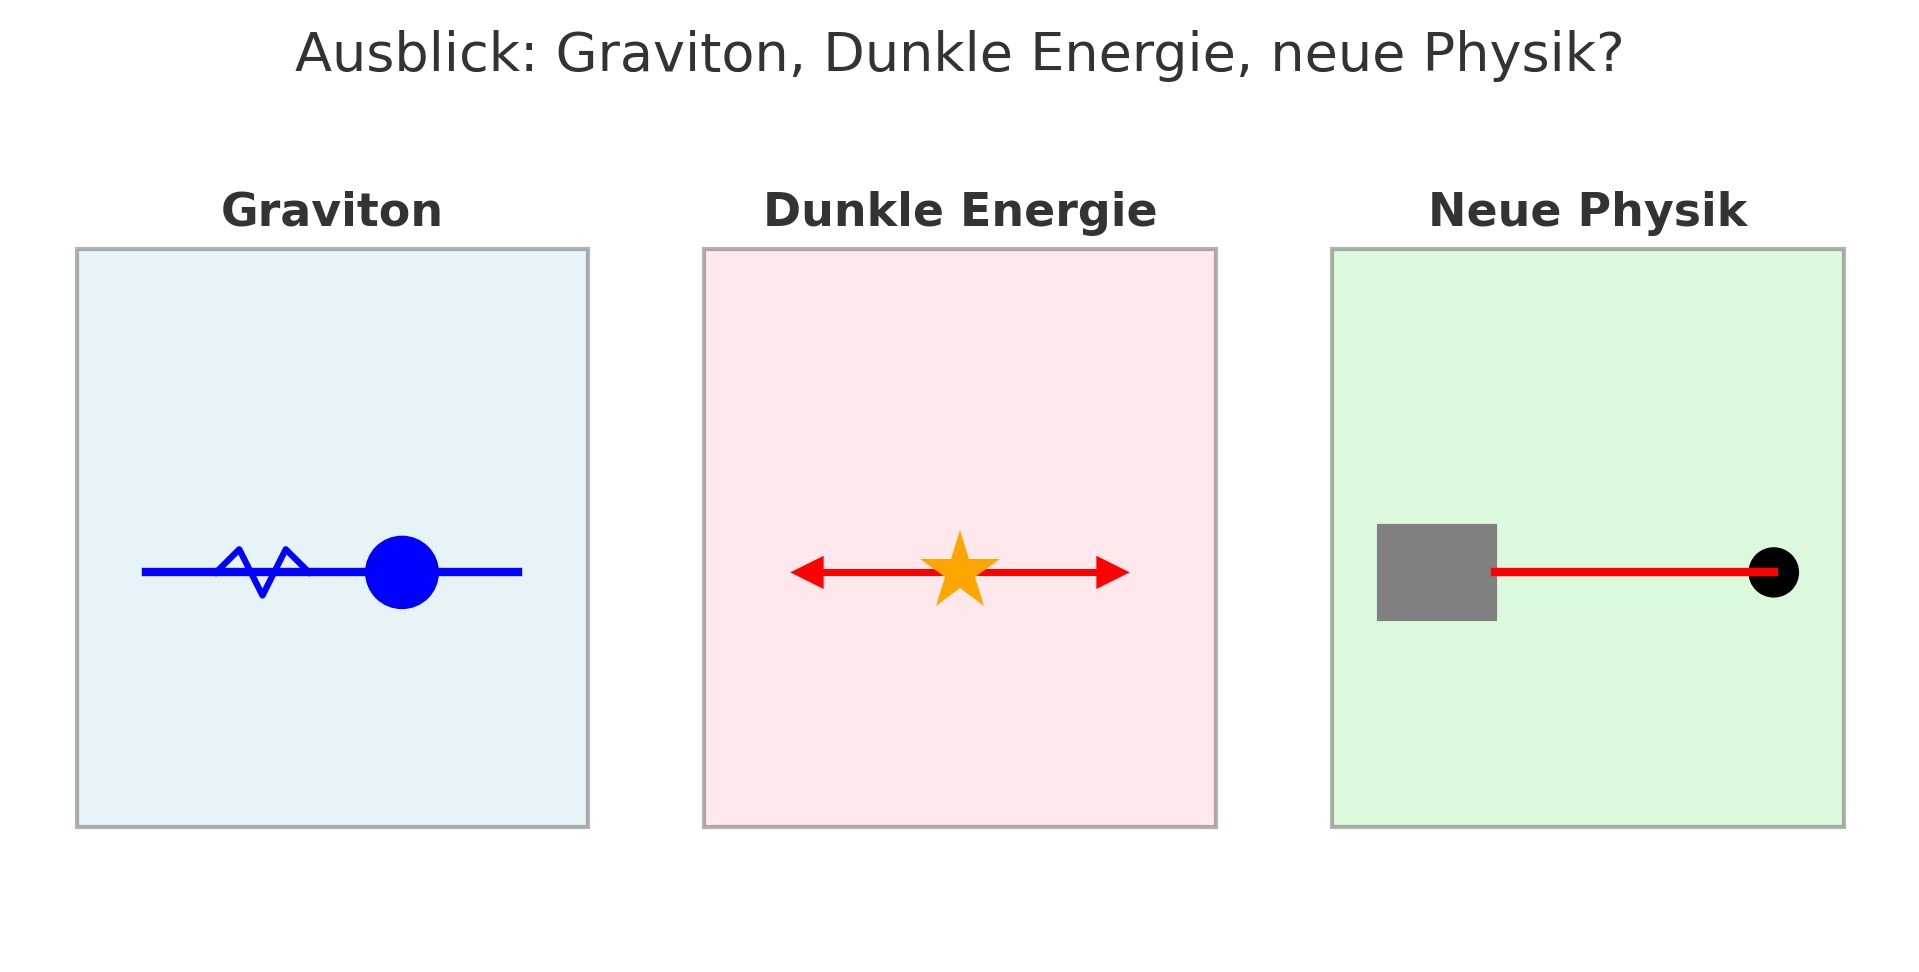
\includegraphics[width=0.9\textwidth]{bilder/photonen_ausblick_fixed.png}
	\caption{Symbolic outlook on open questions in physics:
		\textbf{left:} the hypothetical graviton as a possible candidate for another massless exchange particle;
		\textbf{center:} dark energy, recognizable in the accelerated expansion of the universe;
		\textbf{right:} laboratory experiments with photons searching for hints of new physics.}
	\label{fig:photonen_ausblick}
\end{figure}

\subsubsection{Outlook}

The future of photon research lies not only in technical applications but also in the photon’s role as a precise messenger of new natural laws.  
Space telescopes, gravitational-wave observatories, and laboratory experiments with unprecedented sensitivity could bring us closer to answering these fundamental questions.

\subsection{Conclusion}

Photons are far more than just carriers of light — they are tools, data transmitters, measuring instruments, and messengers of the fundamental laws of nature.  
From optical communication and precision metrology to photonic computers and the study of cosmic phenomena, their versatility is evident.  
The applications presented here make clear that photons not only form the foundation of modern technologies but are also crucial for exploring open questions of physics — from the nature of gravitation and dark energy to possible extensions of the Standard Model.  
The future of photon research therefore lies both in the further development of technical systems and in the search for new physics.

\medskip
\emph{The photon is not just a particle of light — it is a key to today’s technology and to the physics of tomorrow.}
\vspace{1em}
\begin{tcolorbox}[hypobox, title={What If We Could Fully Control Photons?}]
	\label{box:hypo_kapVII}
	A thought experiment: 
	\begin{itemize}
		\item Photonic chips could replace classical electronics — with nearly light-speed computations.
		\item Global quantum communication networks would be absolutely secure against eavesdropping.
		\item Single-photon labs could revolutionize medical diagnostics at the molecular level.
		\item Photons as “probes” could provide direct insights into dark matter or the structure of spacetime.
	\end{itemize}
	\medskip
	Such visionary scenarios go beyond today’s technology — they form the bridge to the next chapter on \emph{The Photon in the Standard Model and Visionary Applications}.
\end{tcolorbox}



